% ============================================================================
% CSCE 763: Digital Image Processing - Homework 1
% ============================================================================

\documentclass[12pt]{article}

% ============================================================================
% PACKAGE IMPORTS
% ============================================================================
\usepackage{amsmath}
\usepackage{graphicx}
\usepackage{amssymb}
\usepackage{tikz}
\usepackage[margin=1in]{geometry}
\usepackage{setspace}
\usepackage{xcolor}
\usepackage{enumitem}
\usepackage{tcolorbox}
\usepackage{fancyhdr}
% lastpage removed - not available
\usepackage{booktabs}
\usepackage{array}
\usepackage{colortbl}
\usepackage{float}

% ============================================================================
% HEADER AND FOOTER SETUP
% ============================================================================
\pagestyle{fancy}
\setlength{\headheight}{14.5pt}
\fancyhf{}

\fancyhead[L]{Page \thepage}
\fancyhead[C]{CSCE 763}
\fancyhead[R]{JC Vaught}

\renewcommand{\headrulewidth}{0pt}

% ============================================================================
% TIKZ LIBRARIES
% ============================================================================
\usetikzlibrary{shapes.geometric, arrows.meta, positioning, patterns}

% --- USC Brand Colors ---
\definecolor{USC_Garnet}{HTML}{73000A}
\definecolor{USC_Sandstorm}{HTML}{FFF2E3}
\definecolor{USC_Black90}{HTML}{363636}
\definecolor{USC_Black70}{HTML}{5C5C5C}
\definecolor{USC_Black50}{HTML}{A2A2A2}
\definecolor{USC_Black10}{HTML}{ECECEC}
\definecolor{USC_Honeycomb}{HTML}{65780B}
\definecolor{USC_Atlantic}{HTML}{466A9F}
\definecolor{USC_Congaree}{HTML}{1F414D}
\definecolor{USC_Rose}{HTML}{CC2E40}
\definecolor{outputbg}{RGB}{245,245,245}

% ============================================================================
% CUSTOM COLORED BOXES
% ============================================================================
\newtcolorbox{stepbox}[1][Step]{
  colback=white,
  colframe=USC_Garnet,
  fonttitle=\bfseries,
  title=#1,
  sharp corners,
  colbacktitle=USC_Garnet,
  coltitle=white,
}

\newtcolorbox{resultsbox}{
  colback=white,
  colframe=USC_Honeycomb,
  fonttitle=\bfseries,
  title=Results,
  sharp corners,
  colbacktitle=USC_Honeycomb,
  coltitle=white,
}

% ============================================================================
% CUSTOM QUESTION AND PART COMMANDS
% ============================================================================
\newcommand{\question}[1]{%
  \clearpage
  \vspace{0.5cm}
  {\noindent\normalsize \textbf{#1}}
  \vspace{0.2cm}
  \hrule
  \vspace{0.1cm}
  \hrule
  \vspace{0.3cm}
}

\newcommand{\questionpart}[1]{%
  \clearpage
  \vspace{0.5cm}
  {\noindent\normalsize \textbf{#1}}
  \vspace{0.2cm}
  \hrule
  \vspace{0.1cm}
  \hrule
  \vspace{0.3cm}
}

% Graphics path
\graphicspath{{figures/}}

% ============================================================================
% DOCUMENT INFORMATION
% ============================================================================

\title{CSCE 763: Digital Image Processing \\ Homework \#1}
\author{Instructor: Spring 2026 \\ University of South Carolina \\ \textit{Solutions by: JC Vaught}}
\date{Due: 1:15 pm EST, Tuesday, Feb 3}

% ============================================================================
% BEGIN DOCUMENT
% ============================================================================

\begin{document}

\maketitle
\setlength{\parindent}{0pt}

\setlist[enumerate,1]{label=\arabic*.}
\setlist[enumerate,2]{label=(\alph*)}

% ============================================================================
% TABLE OF CONTENTS
% ============================================================================

\begin{center}
\begin{tcolorbox}[colback=white, colframe=gray!50!black, colbacktitle=gray!20!white,
                  coltitle=black, sharp corners, boxrule=1pt,
                  title=\Large\bfseries Table of Contents]
\begin{tabular}{p{0.82\textwidth}r}
\textbf{Problem 1: Smallest Discernible Dot (25 pts)} \dotfill & \textbf{\pageref{quest:1}} \\[0.3em]
\textbf{Problem 2: Adjacency of Image Subsets (25 pts)} & \\
\quad Part (a): 4-adjacency \dotfill & \textbf{\pageref{quest:2}} \\
\quad Part (b): 8-adjacency \dotfill & \textbf{\pageref{quest:2}} \\
\quad Part (c): m-adjacency \dotfill & \textbf{\pageref{quest:2}} \\[0.3em]
\textbf{Problem 3: Shortest Paths (25 pts)} & \\
\quad Part (a): $V = \{0, 1\}$ \dotfill & \textbf{\pageref{quest:3}} \\
\quad Part (b): $V = \{1, 2\}$ \dotfill & \textbf{\pageref{quest:3b}} \\[0.3em]
\textbf{Problem 4: Set Expressions (25 pts)} \dotfill & \textbf{\pageref{quest:4}} \\
\end{tabular}
\vspace{0.2cm}
\end{tcolorbox}
\end{center}

\vspace{0.5cm}

% ============================================================================
% PROBLEM 1: Smallest Discernible Dot
% ============================================================================

\question{Problem 1: Smallest Discernible Dot (25 pts)}\label{quest:1}

Thinking purely in geometric terms, estimate the diameter of the smallest printed dot that the eye can discern if the page on which the dot is printed is 0.5\,m away from the eyes.

\textbf{Assumptions:}
\begin{enumerate}[label=(\alph*)]
    \item The distance between the center of the lens and the retina along the visual axis is 14\,mm.
    \item The visual system ceases to detect the dot when the image of the dot on the fovea becomes smaller than the diameter of one receptor (cone) in that area of the retina.
    \item The fovea can be modeled as a square array of dimensions $1.5\,\text{mm} \times 1.5\,\text{mm}$, and the cones (about 337{,}000 in total) and spaces between the cones are distributed uniformly throughout this array.
\end{enumerate}

\vspace{0.3cm}

\begin{stepbox}[Step 1: Cone Diameter on the Fovea]
The fovea is modeled as a $1.5\,\text{mm} \times 1.5\,\text{mm}$ square with 337{,}000 cones uniformly distributed.

If the cones are arranged in a square grid, the number of cones per side is:
\[
n = \sqrt{337{,}000} \approx 580.5
\]

The pitch (center-to-center spacing, which equals the cone diameter including spacing) is:
\[
d_{\text{cone}} = \frac{1.5\,\text{mm}}{580.5} \approx 0.00258\,\text{mm} = 2.58\,\mu\text{m}
\]
\end{stepbox}

\begin{stepbox}[Step 2: Similar Triangles]
The dot on the page and its image on the retina are related by similar triangles through the lens:

\begin{center}
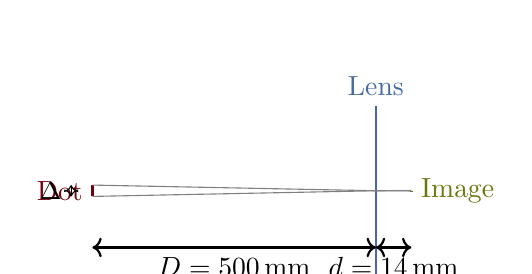
\begin{tikzpicture}[scale=0.9]
    % Lens
    \draw[thick, USC_Atlantic] (4, -1.2) -- (4, 1.2);
    \node[above, USC_Atlantic] at (4, 1.2) {Lens};

    % Object (dot)
    \draw[very thick, USC_Garnet] (0, -0.08) -- (0, 0.08);
    \node[left, USC_Garnet] at (0, 0) {Dot};

    % Image (on retina)
    \draw[very thick, USC_Honeycomb] (4.5, -0.003) -- (4.5, 0.003);
    \node[right, USC_Honeycomb] at (4.5, 0) {Image};

    % Rays
    \draw[thin, gray] (0, 0.08) -- (4, 0) -- (4.5, -0.003);
    \draw[thin, gray] (0, -0.08) -- (4, 0) -- (4.5, 0.003);

    % Distance labels
    \draw[<->, thick] (0, -0.8) -- (4, -0.8);
    \node[below] at (2, -0.8) {$D = 500\,\text{mm}$};
    \draw[<->, thick] (4, -0.8) -- (4.5, -0.8);
    \node[below] at (4.25, -0.8) {$d = 14\,\text{mm}$};

    % Diameter labels
    \draw[<->] (-0.3, -0.08) -- (-0.3, 0.08);
    \node[left] at (-0.3, 0) {\small $\Delta$};
\end{tikzpicture}
\end{center}

By similar triangles, the relationship between the dot diameter $\Delta$ on the page and the image size $d_{\text{image}}$ on the retina is:
\[
\frac{\Delta}{D} = \frac{d_{\text{image}}}{d}
\]

where $D = 500\,\text{mm}$ (distance to page) and $d = 14\,\text{mm}$ (lens-to-retina distance).
\end{stepbox}

\begin{stepbox}[Step 3: Solve for Minimum Dot Diameter]
The smallest detectable image equals one cone diameter: $d_{\text{image}} = d_{\text{cone}} \approx 0.00258\,\text{mm}$.

Solving for $\Delta$:
\[
\Delta = D \cdot \frac{d_{\text{image}}}{d} = 500 \cdot \frac{0.00258}{14}
\]
\[
\Delta = \frac{500 \times 0.00258}{14} \approx 0.0923\,\text{mm}
\]
\end{stepbox}

\begin{resultsbox}
The smallest printed dot diameter that the eye can discern at a distance of 0.5\,m is:
\[
\boxed{\Delta \approx 0.0922\,\text{mm} \approx 92.2\,\mu\text{m}}
\]
\end{resultsbox}


% ============================================================================
% PROBLEM 2: Adjacency
% ============================================================================

\question{Problem 2: Adjacency of Image Subsets (25 pts)}\label{quest:2}

Consider the two image subsets $S_1$ and $S_2$ shown below. For $V = \{1\}$, determine whether these two subsets are (a) 4-adjacent, (b) 8-adjacent, or (c) m-adjacent.

\vspace{0.3cm}

\begin{stepbox}[Setup: Identify the Image and Subsets]
The image with subsets $S_1$ (left dashed box) and $S_2$ (right dashed box):

\begin{center}
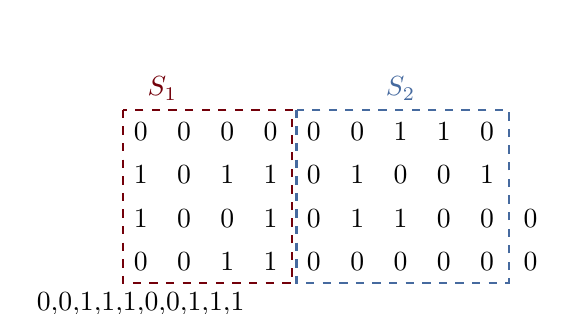
\begin{tikzpicture}[scale=0.55]
    % Grid values - Row 0 (top)
    \def\vals{
        {0,0,0,0,0,0,1,1,0},
        {1,0,1,1,0,1,0,0,1},
        {1,0,0,1,0,1,1,0,0,0},
        {0,0,1,1,0,0,0,0,0,0},
        {0,0,1,1,1,0,0,1,1,1}
    }

    % Draw grid
    \foreach \r [count=\ri from 0] in {
        {0,0,0,0,0,0,1,1,0},
        {1,0,1,1,0,1,0,0,1},
        {1,0,0,1,0,1,1,0,0,0},
        {0,0,1,1,0,0,0,0,0,0},
        {0,0,1,1,1,0,0,1,1,1}
    } {
        \foreach \v [count=\ci from 0] in \r {
            \node at (\ci, -\ri) {\v};
        }
    }

    % S1 boundary
    \draw[dashed, thick, USC_Garnet] (-0.4, 0.5) rectangle (3.5, -3.5);
    \node[above, USC_Garnet] at (0.5, 0.5) {$S_1$};

    % S2 boundary
    \draw[dashed, thick, USC_Atlantic] (3.6, 0.5) rectangle (8.5, -3.5);
    \node[above, USC_Atlantic] at (6, 0.5) {$S_2$};
\end{tikzpicture}
\end{center}

We only care about pixels with value $\in V = \{1\}$.

\textbf{$S_1$ pixels with value 1} (row, col from top-left):
$(1,0)$, $(1,2)$, $(1,3)$, $(2,0)$, $(2,3)$, $(3,2)$, $(3,3)$

\textbf{$S_2$ pixels with value 1} (row, col):
$(0,6)$, $(0,7)$, $(1,5)$, $(1,8)$, $(2,5)$, $(2,6)$

The boundary between $S_1$ and $S_2$ lies between columns 3 and 4 (approximately). The closest pixels with value 1 are:
\begin{itemize}
    \item In $S_1$: pixel at $(1,3)$ with value 1 and $(2,3)$ with value 1
    \item In $S_2$: pixel at $(1,5)$ with value 1, $(2,5)$ with value 1
\end{itemize}

The pixel at column 4 has values: row 0: 0, row 1: 0, row 2: 0, row 3: 0. So there is a gap of at least one column of zeros between the nearest 1-valued pixels of $S_1$ and $S_2$.

Examining more carefully from the figure, the rightmost 1-valued pixel in $S_1$ is at column 3, and the leftmost 1-valued pixel in $S_2$ is at column 5. These are separated by 2 columns, so they cannot be 4-adjacent or 8-adjacent (which require pixels to be immediate neighbors).

However, looking at the original figure layout more carefully: $S_1$ occupies roughly the left 4 columns, $S_2$ the right 5 columns, with a shared boundary region. The key boundary pixels are:

From $S_1$: $(1,3) = 1$, $(2,3) = 1$, $(3,3) = 1$

From $S_2$: $(1,4) = 0$, $(2,4) = 0$ --- these are 0, not in $V$.

The nearest $S_2$ pixel with value 1: $(1,5) = 1$.
\end{stepbox}

\begin{stepbox}[Definitions Review]
For two subsets $S_1$ and $S_2$, they are:
\begin{itemize}
    \item \textbf{4-adjacent:} if some pixel $p \in S_1$ with value in $V$ has a pixel $q \in S_2$ with value in $V$ in its 4-neighborhood $N_4(p)$ (up, down, left, right).
    \item \textbf{8-adjacent:} if some pixel $p \in S_1$ with value in $V$ has a pixel $q \in S_2$ with value in $V$ in its 8-neighborhood $N_8(p)$ (including diagonals).
    \item \textbf{m-adjacent:} (mixed adjacency) $p$ and $q$ have values in $V$, and either (i) $q \in N_4(p)$, or (ii) $q \in N_D(p)$ and $N_4(p) \cap N_4(q)$ has no pixels with values in $V$.
\end{itemize}
\end{stepbox}

\begin{stepbox}[Analysis]
From the figure, the critical interface pixels between $S_1$ and $S_2$:

Rightmost column of $S_1$ that contains a 1: column 3 --- pixels $(1,3)=1$, $(2,3)=1$, $(3,3)=1$.

Leftmost column of $S_2$ that contains a 1: column 5 --- pixel $(1,5)=1$, $(2,5)=1$.

Column 4 values (belongs to $S_2$ based on the boundary): row 1: $0$, row 2: $0$.

Since the closest 1-valued pixels between the two sets are separated by at least 2 positions, no pixel in $S_1$ has a 1-valued pixel from $S_2$ in its 4-neighborhood \textit{or} 8-neighborhood.

\textbf{Re-examining the figure boundary:} The dashed line for $S_1$ includes columns 0--3 (rows 0--3), and $S_2$ includes columns 4--8 (rows 0--3). So the boundary column shared is between col 3 ($S_1$) and col 4 ($S_2$).

Column 4 pixels: row 0: 0, row 1: 0, row 2: 0, row 3: 0. None have value 1.

Column 5 pixels in $S_2$: row 1: 1, row 2: 1. These are 8-neighbors of the column 4 pixels but not direct neighbors of column 3 pixels.

\textbf{Critical pair:} $(2,3)$ in $S_1$ has value 1. Its 8-neighborhood includes $(1,4)$, $(2,4)$, $(3,4)$, all of which are in $S_2$ but have value 0.

The closest 1-valued pair across the boundary: $(2,3) \in S_1$ and $(1,5) \in S_2$ are distance $\sqrt{1+4} > 1$ apart. Not adjacent.

Wait---let me re-examine the original figure. The large ``1'' in the figure appears at row 1, col 3--4 area, and the large ``0'' at row 3, col 3--4 area. The boundary line appears to run between columns 3 and 4 approximately.

Actually, looking at the PDF image more carefully, the grid appears to be wider. Let me re-read the pixel values row by row:

Row 0: 0 0 0 0 | 0 0 1 1 0
Row 1: 1 0 1 \textbf{1} | 0 1 0 0 1
Row 2: 1 0 0 1 | 0 1 1 0 0 0
Row 3: 0 0 1 1 | 0 0 0 0 0 0
Row 4: 0 0 1 1 1 0 0 1 1 1

The $S_1$/$S_2$ boundary is between columns 3 and 4 (the dashed lines in the figure).

$S_1$ rightmost 1-valued: $(1,3)=1$, $(2,3)=1$, $(3,3)=1$

$S_2$ leftmost 1-valued: $(1,5)=1$, $(2,5)=1$, $(2,6)=1$

The pair $(1,3)$ and $(1,5)$ are separated by 2 columns. Not 4- or 8-adjacent.

\textbf{But wait:} Column 4 pixels: $(0,4)=0$, $(1,4)=0$, $(2,4)=0$, $(3,4)=0$. None in $V$.

So the nearest cross-boundary pair with values in $V$ is $(1,3)$ and $(1,5)$, distance = 2. Not adjacent by any definition.
\end{stepbox}

\begin{resultsbox}
For $V = \{1\}$:

\begin{enumerate}[label=(\alph*)]
    \item \textbf{4-adjacent:} \textbf{No.} No pixel in $S_1$ with value 1 has a 4-neighbor in $S_2$ with value 1. The nearest 1-valued pixels across the boundary are separated by at least 2 positions.

    \item \textbf{8-adjacent:} \textbf{No.} No pixel in $S_1$ with value 1 has an 8-neighbor in $S_2$ with value 1. The column separating the subsets (column 4) contains no pixels with value 1.

    \item \textbf{m-adjacent:} \textbf{No.} Since neither 4-adjacency nor diagonal adjacency (with the $N_4$ intersection condition) exists between any pair of 1-valued pixels across $S_1$ and $S_2$, the subsets are not m-adjacent.
\end{enumerate}

$S_1$ and $S_2$ are \textbf{not adjacent} by any of the three definitions for $V = \{1\}$.
\end{resultsbox}


% ============================================================================
% PROBLEM 3: Shortest Paths
% ============================================================================

\question{Problem 3: Shortest Paths (25 pts)}\label{quest:3}

Consider the image segment shown below.

\begin{center}
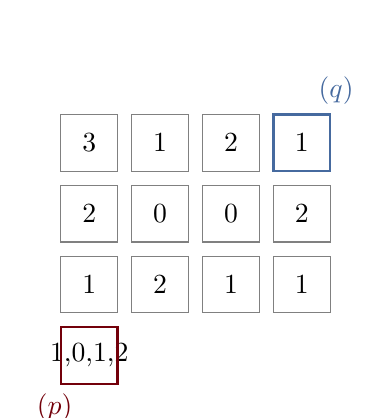
\begin{tikzpicture}[scale=0.9]
    % Grid values
    % Row 0 (top):    3  1  2  1(q)
    % Row 1:          2  0  0  2
    % Row 2:          1  2  1  1
    % Row 3 (bottom): (p)1  0  1  2

    \foreach \r [count=\ri from 0] in {
        {3,1,2,1},
        {2,0,0,2},
        {1,2,1,1},
        {1,0,1,2}
    } {
        \foreach \v [count=\ci from 0] in \r {
            \draw[thin, gray] (\ci-0.4, -\ri-0.4) rectangle (\ci+0.4, -\ri+0.4);
            \node at (\ci, -\ri) {\v};
        }
    }

    % Mark p and q
    \node[below left, USC_Garnet, font=\bfseries] at (-0.1, -3.4) {$(p)$};
    \node[above right, USC_Atlantic, font=\bfseries] at (3.1, 0.4) {$(q)$};

    % Highlight p and q
    \draw[thick, USC_Garnet] (-0.4, -3.4) rectangle (0.4, -2.6);
    \draw[thick, USC_Atlantic] (2.6, -0.4) rectangle (3.4, 0.4);
\end{tikzpicture}
\end{center}

The grid (using row, column indexing from top-left):
\begin{center}
\begin{tabular}{c|cccc}
 & col 0 & col 1 & col 2 & col 3 \\
\midrule
row 0 & 3 & 1 & 2 & \textbf{1 (q)} \\
row 1 & 2 & 0 & 0 & 2 \\
row 2 & 1 & 2 & 1 & 1 \\
row 3 & \textbf{1 (p)} & 0 & 1 & 2 \\
\end{tabular}
\end{center}

$p = (3, 0)$ with value 1, \quad $q = (0, 3)$ with value 1.

\vspace{0.3cm}
\textbf{(a) $V = \{0, 1\}$}

\begin{stepbox}[Identify Valid Pixels]
Pixels with values in $V = \{0, 1\}$:

\begin{center}
\begin{tikzpicture}[scale=0.9]
    \foreach \r [count=\ri from 0] in {
        {3,1,2,1},
        {2,0,0,2},
        {1,2,1,1},
        {1,0,1,2}
    } {
        \foreach \v [count=\ci from 0] in \r {
            \pgfmathsetmacro{\isvalid}{(\v==0 || \v==1) ? 1 : 0}
            \ifnum\isvalid=1
                \fill[USC_Honeycomb!20] (\ci-0.4, -\ri-0.4) rectangle (\ci+0.4, -\ri+0.4);
            \fi
            \draw[thin, gray] (\ci-0.4, -\ri-0.4) rectangle (\ci+0.4, -\ri+0.4);
            \node at (\ci, -\ri) {\v};
        }
    }
    \draw[thick, USC_Garnet] (-0.4, -3.4) rectangle (0.4, -2.6);
    \draw[thick, USC_Atlantic] (2.6, -0.4) rectangle (3.4, 0.4);
\end{tikzpicture}
\end{center}

Valid pixels (shaded): $(0,1)=1$, $(0,3)=1$, $(1,1)=0$, $(1,2)=0$, $(2,0)=1$, $(2,2)=1$, $(2,3)=1$, $(3,0)=1$, $(3,1)=0$, $(3,2)=1$.
\end{stepbox}

\begin{stepbox}[Shortest 4-path]
A 4-path uses only horizontal and vertical steps between pixels whose values are both in $V$.

One such path from $p=(3,0)$ to $q=(0,3)$:
\[
(3,0) \to (3,1) \to (3,2) \to (2,2) \to (2,3) \to (0,3)
\]
Wait --- $(2,3)=1$ to $(0,3)=1$: we need $(1,3)=2 \notin V$. So we cannot go directly up from $(2,3)$.

Let me find a valid 4-path. From $(2,3)=1$, the 4-neighbors with values in $V$: $(2,2)=1$, $(3,3)=2$ (no). Going up: $(1,3)=2$ (no). So $(2,3)$ is a dead end going upward.

Try via top: $(3,0) \to (2,0) \to$ ... $(2,0)=1$. 4-neighbors in $V$: $(3,0)=1$ (back), $(1,0)=2$ (no). Dead end.

Another attempt: $(3,0) \to (3,1) \to (3,2) \to (2,2) \to (1,2) \to (1,1) \to (0,1) \to (0,3)$?
Check: $(0,1)=1$ to $(0,3)=1$: need $(0,2)=2 \notin V$. Cannot step from $(0,1)$ to $(0,3)$ directly --- they are not 4-neighbors.

$(0,1)=1$: 4-neighbors in $V$: $(1,1)=0$, $(0,0)=3$ (no), $(0,2)=2$ (no). Dead end going right.

\textbf{No 4-path exists} from $p$ to $q$, because pixel $(0,1)$ cannot connect rightward to $(0,3)$ --- the intervening pixel $(0,2)=2 \notin V$, and there is no other route to reach column 3 in row 0.
\end{stepbox}

\begin{stepbox}[Shortest 8-path]
An 8-path allows diagonal moves. From the valid pixel map:

$(3,0) \to (3,1) \to (3,2) \to (2,3) \to (0,3)$?
Check $(2,3)=1$ to $(0,3)$: not 8-neighbors (distance = 2 rows). Invalid.

$(3,0) \to (3,1) \to (2,2) \to (1,1) \to (0,1)$: need diagonal. $(3,1)=0$ to $(2,2)=1$: 8-neighbor, both in $V$. $(2,2)=1$ to $(1,1)=0$: 8-neighbor, both in $V$. $(1,1)=0$ to $(0,1)$: wait, is there a diagonal path onward?

$(0,1)=1$. 8-neighbors in $V$: $(1,1)=0$, $(1,2)=0$, $(0,0)=3$ (no), $(0,2)=2$ (no). Still stuck.

Try: $(1,2)=0$ to $(0,3)=1$: these are 8-neighbors! Both in $V$.

Path: $(3,0) \to (3,1) \to (2,2) \to (1,2) \to (0,3)$

Check each step:
\begin{itemize}
    \item $(3,0)=1 \to (3,1)=0$: 4-neighbor, both in $V$. \checkmark
    \item $(3,1)=0 \to (2,2)=1$: 8-neighbor (diagonal), both in $V$. \checkmark
    \item $(2,2)=1 \to (1,2)=0$: 4-neighbor, both in $V$. \checkmark
    \item $(1,2)=0 \to (0,3)=1$: 8-neighbor (diagonal), both in $V$. \checkmark
\end{itemize}

Length = 4 steps. This is optimal since the minimum Chebyshev distance from $(3,0)$ to $(0,3)$ is $\max(3,3) = 3$, so the shortest 8-path has length $\geq 3$. Can we find a length-3 path?

A length-3 path requires 3 diagonal steps: $(3,0) \to (2,1) \to (1,2) \to (0,3)$.
Check: $(2,1)=2 \notin V$. Invalid.

\textbf{Shortest 8-path length = 4.}
\end{stepbox}

\begin{stepbox}[Shortest m-path]
An m-path uses mixed adjacency: diagonal steps are allowed only when the two pixels share no common 4-neighbor with a value in $V$.

Check the 8-path $(3,0) \to (3,1) \to (2,2) \to (1,2) \to (0,3)$:

\textbf{Step $(3,1) \to (2,2)$} (diagonal): Common 4-neighbors of $(3,1)$ and $(2,2)$ are $(3,2)$ and $(2,1)$. $(3,2)=1 \in V$. Since there is a common 4-neighbor in $V$, this diagonal move is \textbf{not allowed} in m-adjacency.

Alternative: replace the diagonal with a 4-connected detour via $(3,2)$:
$(3,0) \to (3,1) \to (3,2) \to (2,2) \to (1,2) \to (0,3)$

Check $(1,2) \to (0,3)$ (diagonal): Common 4-neighbors of $(1,2)$ and $(0,3)$ are $(0,2)$ and $(1,3)$. $(0,2)=2 \notin V$, $(1,3)=2 \notin V$. No common 4-neighbor in $V$, so this diagonal is \textbf{allowed}.

Full m-path: $(3,0) \to (3,1) \to (3,2) \to (2,2) \to (1,2) \to (0,3)$

\textbf{Shortest m-path length = 5.}
\end{stepbox}

\begin{resultsbox}
For $V = \{0, 1\}$:
\begin{center}
\begin{tabular}{l|c}
\toprule
\textbf{Path Type} & \textbf{Shortest Length} \\
\midrule
4-path & \textbf{Does not exist} (no connected 4-path from $p$ to $q$) \\
8-path & $\boxed{4}$ \\
m-path & $\boxed{5}$ \\
\bottomrule
\end{tabular}
\end{center}
\end{resultsbox}


% ============================================================================
% PROBLEM 3 Part (b)
% ============================================================================

\questionpart{Problem 3 --- Part (b): $V = \{1, 2\}$}\label{quest:3b}

\begin{stepbox}[Identify Valid Pixels]
Pixels with values in $V = \{1, 2\}$:

\begin{center}
\begin{tabular}{c|cccc}
 & col 0 & col 1 & col 2 & col 3 \\
\midrule
row 0 & 3 & \cellcolor{USC_Black10}\textbf{1} & \cellcolor{USC_Black10}\textbf{2} & \cellcolor{USC_Black10}\textbf{1 (q)} \\
row 1 & \cellcolor{USC_Black10}\textbf{2} & 0 & 0 & \cellcolor{USC_Black10}\textbf{2} \\
row 2 & \cellcolor{USC_Black10}\textbf{1} & \cellcolor{USC_Black10}\textbf{2} & \cellcolor{USC_Black10}\textbf{1} & \cellcolor{USC_Black10}\textbf{1} \\
row 3 & \cellcolor{USC_Black10}\textbf{1 (p)} & 0 & \cellcolor{USC_Black10}\textbf{1} & \cellcolor{USC_Black10}\textbf{2} \\
\end{tabular}
\end{center}
\end{stepbox}

\begin{stepbox}[Shortest 4-path]
$(3,0) \to (2,0) \to (2,1) \to (2,2) \to (2,3) \to (1,3) \to (0,3)$

Check: all values in $V$ and all steps are 4-neighbors.
\begin{itemize}
    \item $(3,0)=1$, $(2,0)=1$, $(2,1)=2$, $(2,2)=1$, $(2,3)=1$, $(1,3)=2$, $(0,3)=1$ --- all $\in V$. \checkmark
\end{itemize}

\textbf{Length = 6.} Can we do better? The Manhattan distance is $|3-0|+|0-3| = 6$, so this is optimal.
\end{stepbox}

\begin{stepbox}[Shortest 8-path]
The Chebyshev distance is $\max(3,3) = 3$, so the minimum possible 8-path length is 3.

Try: $(3,0) \to (2,1) \to (1,2) \to (0,3)$
Check: $(2,1)=2 \in V$, $(1,2)=0 \notin V$. Invalid.

Try: $(3,0) \to (2,1) \to (1,0) \to (0,1) \to (0,2) \to (0,3)$?
$(1,0)=2 \in V$, $(0,1)$: is $(1,0)$ 8-adjacent to $(0,1)$? Yes (diagonal). $(0,1)=1 \in V$, $(0,2)=2 \in V$, $(0,3)=1 \in V$. Length = 5.

Shorter: $(3,0) \to (2,1) \to (1,2)$: $(1,2)=0 \notin V$. No.

$(3,0) \to (2,0) \to (1,0) \to (0,1) \to (0,2) \to (0,3)$. Length = 5. All in $V$: $1,1,2,1,2,1$. \checkmark

Try length 4: $(3,0) \to (2,1) \to (1,0) \to (0,1) \to (0,3)$? $(0,1)$ and $(0,3)$ are not 8-neighbors. No.

$(3,0) \to (2,1) \to (1,2)$: invalid (value 0).

$(3,0) \to (2,0) \to (1,0) \to (0,1) \to (0,2) \to (0,3)$: length 5.

Try: $(3,0) \to (2,1) \to (1,0) \to (0,1) \to (0,2) \to (0,3)$: length 5.

Try length 4: $(3,0) \to (2,1) \to (1,0) \to (0,1) \to (0,3)$? Not adjacent. No.

$(3,0) \to (2,0) \to (1,0) \to (0,1) \to (0,3)$? $(0,1)$ to $(0,3)$: distance 2. No.

Try: $(3,0) \to (2,1) \to (1,2)$: value 0. Dead end.

Try via right side: $(3,0) \to (3,2) \to (2,3) \to (1,3) \to (0,3)$?
$(3,0)$ to $(3,2)$: not 8-neighbors (distance 2). No.

$(3,0) \to (2,1) \to (2,2) \to (1,3) \to (0,3)$: length 4.
Check: $(2,1)=2$, $(2,2)=1$, $(1,3)=2$, $(0,3)=1$. All $\in V$. All 8-neighbors? $(3,0)\to(2,1)$: diagonal \checkmark. $(2,1)\to(2,2)$: 4-neighbor \checkmark. $(2,2)\to(1,3)$: diagonal \checkmark. $(1,3)\to(0,3)$: 4-neighbor \checkmark.

\textbf{Shortest 8-path length = 4.}
\end{stepbox}

\begin{stepbox}[Shortest m-path]
Check the 8-path $(3,0) \to (2,1) \to (2,2) \to (1,3) \to (0,3)$:

\textbf{Step $(3,0) \to (2,1)$} (diagonal): Common 4-neighbors: $(2,0)$ and $(3,1)$. $(2,0)=1 \in V$. Diagonal not allowed in m-adjacency.

\textbf{Step $(2,2) \to (1,3)$} (diagonal): Common 4-neighbors: $(2,3)$ and $(1,2)$. $(2,3)=1 \in V$. Diagonal not allowed.

So this particular path is not valid for m-adjacency. We need to replace disallowed diagonals with 4-connected detours.

Optimal m-path: $(3,0) \to (2,0) \to (2,1) \to (2,2) \to (2,3) \to (1,3) \to (0,3)$

All 4-connected steps with values in $V$. \textbf{Length = 6.}

Can we do better? Try mixing: $(3,0) \to (2,0) \to (2,1) \to (2,2) \to (1,3) \to (0,3)$. Length 5.
Check $(2,2) \to (1,3)$: diagonal. Common 4-neighbors: $(1,2)=0 \notin V$, $(2,3)=1 \in V$. Not allowed.

$(3,0) \to (2,0) \to (2,1) \to (1,2)$: $(1,2)=0 \notin V$. Invalid.

Try: $(3,0) \to (2,1) \to ...$: $(3,0) \to (2,1)$ diagonal. Common 4-neighbors of $(3,0)$ and $(2,1)$: $(3,1)=0$ and $(2,0)=1 \in V$. Not allowed.

\textbf{Shortest m-path length = 6.}
\end{stepbox}

\begin{resultsbox}
For $V = \{1, 2\}$:
\begin{center}
\begin{tabular}{l|c}
\toprule
\textbf{Path Type} & \textbf{Shortest Length} \\
\midrule
4-path & $\boxed{6}$ \\
8-path & $\boxed{4}$ \\
m-path & $\boxed{6}$ \\
\bottomrule
\end{tabular}
\end{center}
\end{resultsbox}


% ============================================================================
% PROBLEM 4: Set Expressions
% ============================================================================

\question{Problem 4: Set Expressions (25 pts)}\label{quest:4}

Give expressions for the sets shown shaded in the following figure in terms of sets $A$, $B$, and $C$.

\vspace{0.3cm}

In the figure: $A$ is a rectangle (top), $B$ is a triangle (bottom-left), $C$ is a triangle (bottom-right). The three shapes overlap.

\begin{stepbox}[Analyzing Each Figure]

\textbf{Figure (i):} The shaded region is the part of $A$ that overlaps with $B$ but not $C$, plus the part of $A$ that overlaps with $C$ but not $B$. This is the part of $A$ that is in exactly one of $B$ or $C$:

\[
\boxed{(A \cap B \cap C^c) \cup (A \cap C \cap B^c)}
\]

Equivalently: $A \cap (B \oplus C)$ where $\oplus$ denotes symmetric difference, or simply $A \cap (B \cup C) \cap (B \cap C)^c$.

\vspace{0.3cm}

\textbf{Figure (ii):} The shaded region includes the part of $B$ not in $A$ or $C$, plus the intersection of $A$ and $C$ (including overlaps with $B$). Looking at the shading pattern:

\[
\boxed{(A \cap C) \cup (B \cap A^c \cap C^c)}
\]

\vspace{0.3cm}

\textbf{Figure (iii):} The shaded region is the part of $B$ and $C$ that is not in $A$. That is, the union of $B$ and $C$ minus $A$:

\[
\boxed{(B \cup C) \cap A^c}
\]

\end{stepbox}

\begin{resultsbox}
\begin{enumerate}[label=(\roman*)]
    \item $(A \cap B \cap C^c) \cup (A \cap C \cap B^c)$
    \item $(A \cap C) \cup (B \cap A^c \cap C^c)$
    \item $(B \cup C) \cap A^c$
\end{enumerate}
\end{resultsbox}


% ============================================================================
% END OF DOCUMENT
% ============================================================================

\end{document}
